\begin{appendices}

%\appendixpage
%\addappheadtotoc

\section{技术详解:去信任的清算协议}\label{sec:codes}
本节具体阐述闪电网络清算协议的技术细节。对于技术细节不感兴趣的读者可以略过此部分,只需阅读\ref{sec:clearing}。

闪电网络的技术细节晦涩难懂,而且工程实现的复杂度也比较大。部分原因是由于闪电网络的清算协议基于比特币协议,其智能合约是通过堆栈式指令编写,类似于汇编语言的风格。而以太坊的智能合约编程语言 Solidity 的语法接近于 JavaScript,是一种高级编程语言的风格,相对来讲有更好的可读性。所以本文基于 Solidty 重新表达闪电网络协议。在保持技术原理一致性的前提下,尽量提高可读性,帮助读者降低学习的门槛。

\subsection{虚拟银行智能合约}

不失一般性,假设 Alice 和 Bob 两个用户在某一段时间内需要频繁的往来支付。
于是双方协商建立共同的虚拟银行智能合约。
这个合约模拟了一个微型银行,只有 Alice 和 Bob 两个账户。
双方约定分别在虚拟银行中存入 100 美元,用 [100, 100] 表示 Alice 和 Bob 在资产负债表的初始余额。

虚拟银行智能合约的源码位于:\href{https://github.com/dapenghu/solidity-bidirection-payment-channel/blob/master/virtualBank/contracts/VirtualBank.sol}{GitHub: Solidity Bidirection Payment Channel}。

\subsubsection{合约数据结构}
首先介绍虚拟银行的数据结构,一共分为三部分:

\begin{itemize}
    \item 虚拟银行状态 State \_state。
        虚拟银行一共有4个状态,如下图所示。
        \begin{figure}[h!]
            \centering
            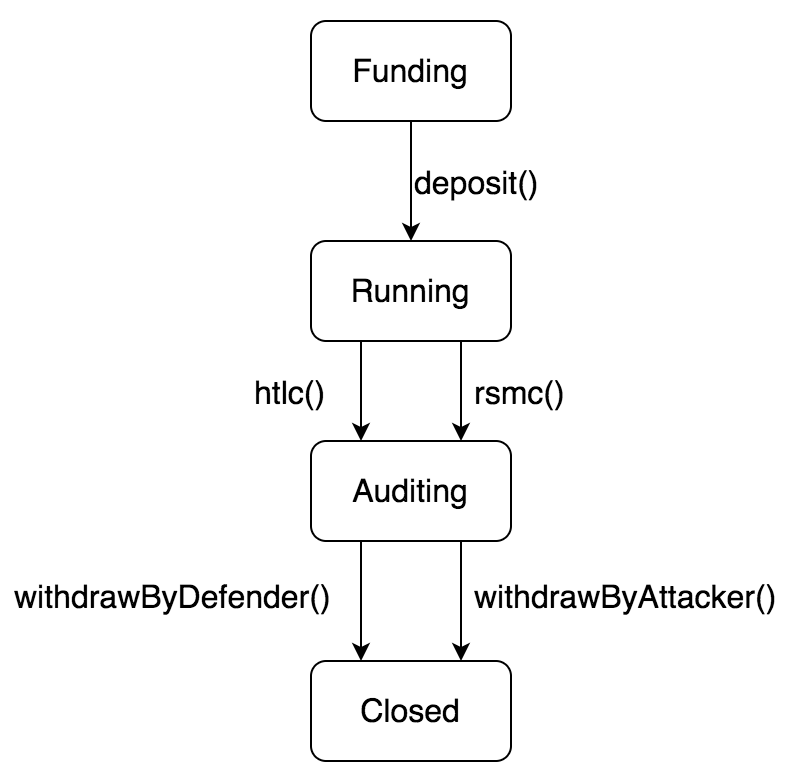
\includegraphics[width=12cm, keepaspectratio]{../images/state_machine.png}
            \caption{虚拟银行状态变换}
            \label{fig:A_state_machince}
        \end{figure}
        \begin{enumerate}
            \item Funding: 智能合约初始化完成之后进入 Funding 状态,Alice 和 Bob 根据约定的额度,调用depoit() 往虚拟银行里转账。Alice 和 Bob 都足额注入100美金之后,虚拟银行进入 Running 状态。
            \item Running: 此时,Alice 和 Bob 在链下可以进行微支付交易。他们随时可以提交资产承诺提案(虚拟银行接受 RSMC、HTLC 两种提案)。虚拟银行将根据承诺提案的条款,立刻结算防御方的资产,冻结进攻方的资产作为诚信保证金。然后进入 Auditing 状态。
            \item Auditing: 在诚信保证金冻结期间,防御方可以检查承诺是否被撤销。如果是,那么他可以取走诚信保证金;否则进攻方可以在冻结期满之后,可以取回诚信保证金。无论哪种情况,虚拟银行都会进入 Closed 状态。
            \item Closed: 虚拟银行的所有资产都已结清,支付通道随之关闭。
        \end{enumerate}

    \item 用户数据 Client[2] \_clients。
    
    由于虚拟银行只有两个账户: Alice 和 Bob。所以此数组的长度永远是 2。每一项保存的用户的地址、应存入的余额,以及是否已经足额存款。
    
    \item 承诺数据 Commitment \_commitment
    
    变量 \_commitment 记录 Alice 和 Bob 双方已经约定的承诺,包含如何分配虚拟银行的资产,以及承诺编号、进攻方、撤销锁、诚信保证金的冻结时间等。
    
\end{itemize}
\begin{lstlisting}[caption={虚拟银行智能合约数据结构.}, label={lst:data}]
/**
* @title Virtual bank smart contract. Support RSMC and HTLC commitments.
* @dev Simulate the lightning network clearing protocol with Solidity programming language.
*/
contract VirtualBank {
    using SafeMath for uint256;
    using ECRecovery for bytes32;
    string[2] constant NAMES = [string("Alice"), "Bob"];
    struct Client {
        address addr;   // Alice's and Bob's addresses
        uint256 amount;      // amount of each account
        bool    deposited;   // whether each account deposit enough fund
    }
    struct Commitment {
        uint32     sequence;
        uint8      attacker;      // defender = 1 - attacker
        address    revocationLock;
        uint       freezeTime;
        uint       requestTime;
        uint256[2] amounts;        // amount[attacker] is fidelity bond
    }
    // enum for virtual bank state
    enum State { Funding, Running, Auditing, Closed }
    // balance sheets
    Client[2] _clients;
    // state of virtual bank
    State _state;
    // commitment data
    Commitment _commitment;
}
\end{lstlisting}


\subsubsection{构造函数}

创建虚拟银行之前,Alice 和 Bob 需要提前协商相关的配置参数,这些参数包括:

1. Alice 和 Bob 的个人账户地址: address[2] addrs。
2. Alice 和 Bob 欲存入的账户余额。

构造函数检查输入参数的合法性,初始化用户数据 \_clients, 和承诺方案 \_commitment 之后,进入 Funding 状态。

\begin{lstlisting}[caption={构造函数.}, label={lst:constructor}]
/**
 * @notice The contructor of virtual bank smart contract
 * @param addrs  Addresses of Alice and Bob
 * @param amount Balance amount of Alice and Bob
 */
constructor(address[2] addrs, uint256[2] amounts) public 
    validAddress(addrs[0])  validAddress(addrs[1]){
    Client alice = Client(addrs[0], amounts[0], false);
    Client bob   = Client(addrs[1], amounts[1], false);
    _clients = [Client(alice), bob];
    
    _commitment = Commitment(0, 0, address(0), 0, 0, new uint256[](2));
    _state = State.Funding;
    emit VirtualBankFunding(alice.addr, alice.amount, bob.addr, bob.amount);
}
\end{lstlisting}

\subsubsection{资金存款}
在虚拟银行的 Funding 状态,Alice 和 Bob 调用 deposit() 函数向银行转入预订额度的资金。双方的资金都转入之后,虚拟银行进入 Running 状态。双向支付通道搭建完成,Alice 和 Bob 现在可以使用 RSMC承诺方案 或者 HTLC 承诺方案进行多笔微支付。

\begin{lstlisting}[caption={存款}, label={lst:deposit}]
/**
 * @notice Alice or Bob deposit fund to virtual bank.
 */
function deposit()  external payable isFunding() {

    if(msg.sender == _clients[0].addr 
    && msg.value == _clients[0].amount 
    && !_clients[0].deposited) {
        _clients[0].deposited = true;
        emit Deposit("Alice", msg.sender, msg.value);
    } else if (msg.sender == _clients[1].addr 
            && msg.value == _clients[1].amount 
            && !_clients[1].deposited) {
        _clients[1].deposited = true;
        emit Deposit("Bob", msg.sender, msg.value);
    } else {
        throw;
    }
    // If both Alice and Bob have deposited fund, virtual bank begin running.
    if (_clients[0].deposited && _clients[1].deposited) {
        _state = State.Running;
        emit VirtualBankRunning(_clients[0].addr, _clients[0].amount, 
                                _clients[1].addr, _clients[1].amount);
    }
}

\end{lstlisting}

\subsection{RSMC 承诺方案}

RSMC 承诺方案是最简单、也是最基础的承诺方案。
它是 Alice 和 Bob 对于虚拟银行中的资产如何分配达成的相互承诺。
虚拟银行的资产清算可以通过 RSMC 承诺方案实现。
由于承诺的协商和更新只需要 Alice 和 Bob 双方参与,不需要众多的矿工参与共识,从而实现价值的传递可以快速的完成。

\subsubsection{RSMC 承诺方案数据结构}
根据 \ref{sec:commiment} 节所述:RSMC 承诺方案具有不可伪造性、不可篡改性、可以撤销性。
RSMC 协议模拟了银行资产清算的过程。
每一次支付会重新产生一份新的承诺方案,经过一段时间的积累,Alice 和 Bob 会有多份资产清算方案,但是只有最后的方案才是有效的结果。
每一个 RSMC 承诺方案都有一个唯一编号。每生成一个新的承诺方案,编号加一。
任何时候,编号最大的承诺是有效的,其它的历史承诺方案都已经被撤销。

如下图 \ref{fig:rsmc_3} 所示,从虚拟银行建立之后,Alice 和 Bob 一共达成 N 次共同承诺,当前有效的承诺编号为 N,之前编号更低的承诺都已经被撤销。

\begin{figure}[h!]
    \centering
    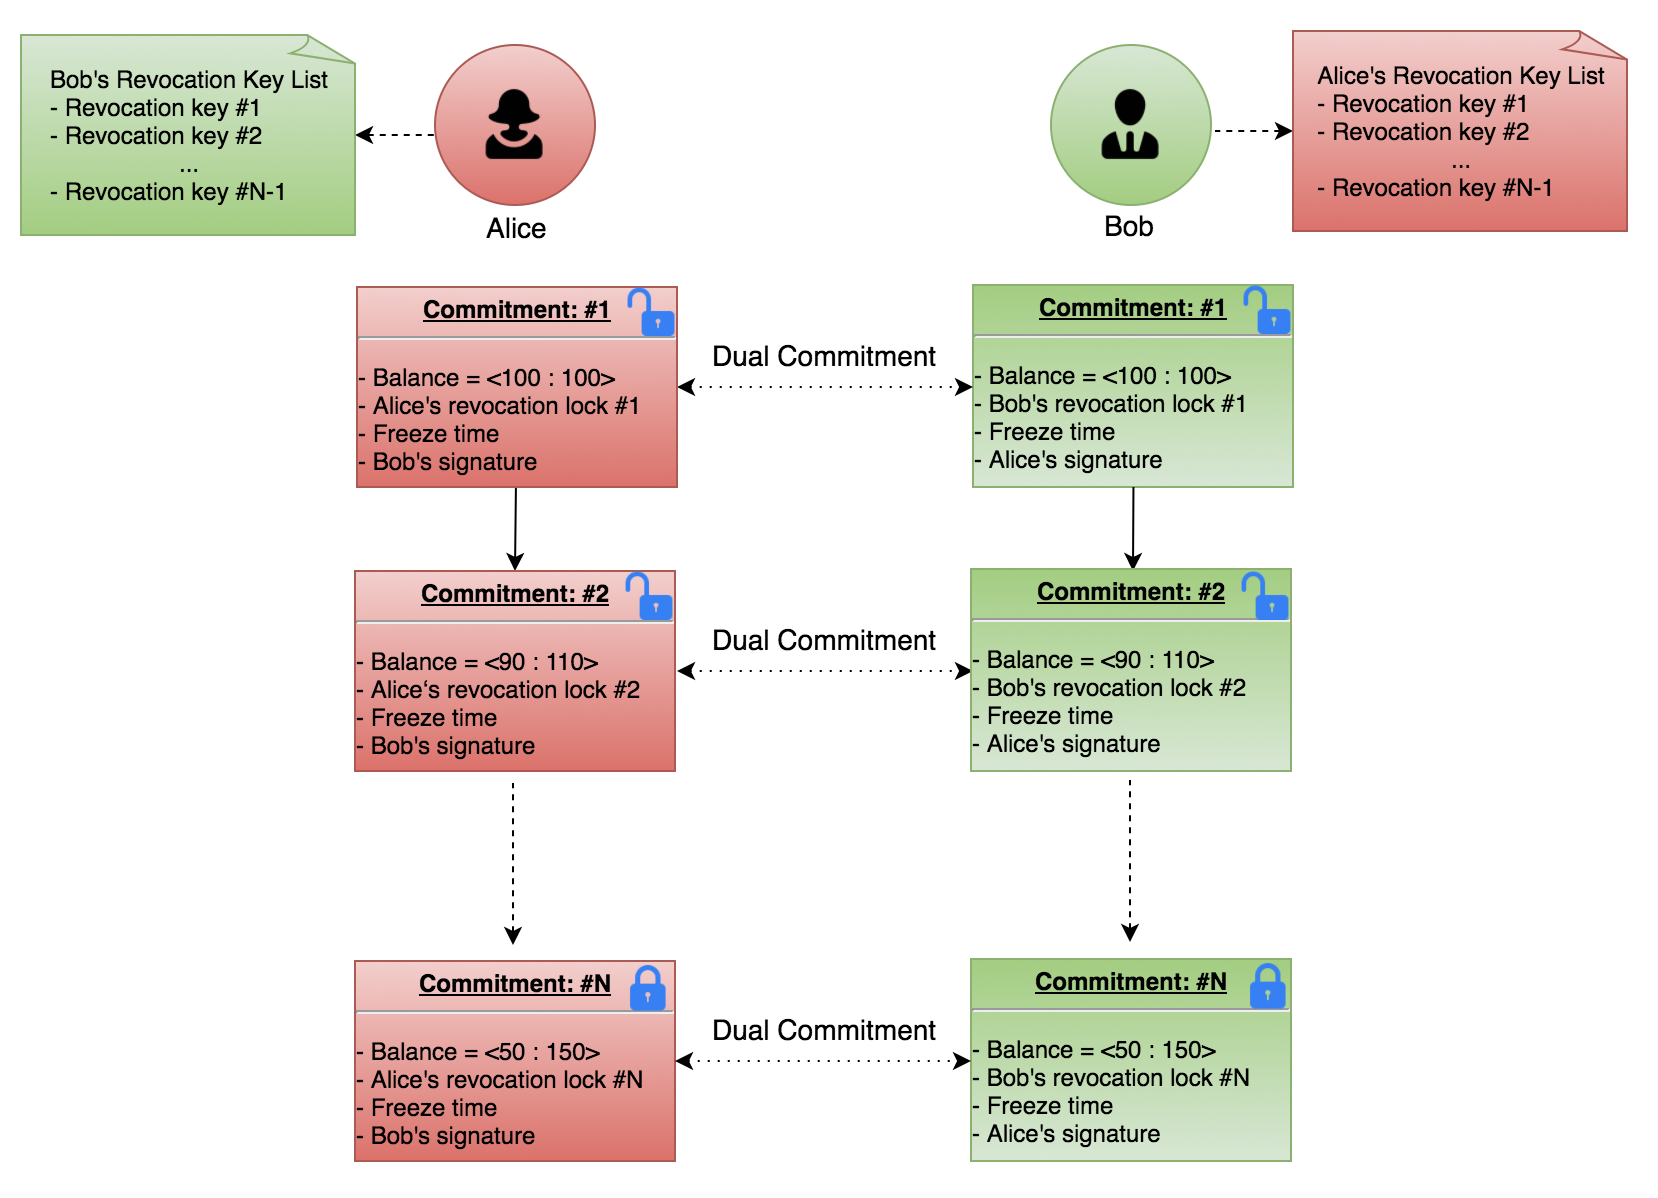
\includegraphics[width=12cm, keepaspectratio]{../images/dual_rsmc_3.png}
    \caption{RSMC 承诺方案}
    \label{fig:A_rsmc_3}
\end{figure}

另外注意到,每一次承诺有左右两份,互为对偶承诺,二者的资产负债表和诚信保证金的冻结时间是一样的。
但是攻守双方的位置互换。左面的承诺以 Alice 为进攻方,撤销锁是 Alice 生成的,初审的签名由Bob签署;
反之,右面的承诺以 Bob 为进攻方,撤销锁是 Bob 生成的,初审签名由 Alice 签署。

这些承诺方案还只有防御方的签名,没有进攻方的签名,处于未兑现状态。
如果某一方想兑现承诺,取出虚拟银行中的资产,可以签署自己手里的那一份承诺方案,然后广播到链上。
虚拟银行智能合约收到后会按照承诺中约定的方式结算双方的资产。

下面按照支付通道的建立,使用,关闭三个环节介绍 RSMC 承诺方案的使用过程。

\subsubsection{创建支付通道}
依然假设 Alice 和 Bob 要创建一个支付通道,要经过4个步骤:
\begin{enumerate}
    \item 预备阶段:双方交换如下信息
        \begin{itemize}
            \item 交换彼此的账户地址 
            \item 确定各自的出资额度: 比如 Alice 计划出资 100 美元, Bob 也出资 100 美元。
            \item 协商诚信保证金的锁定时间(FreezeTime)
            \item 提前交换一批撤销锁。比如先交换编号 1-100 的撤销锁。只是交换撤销锁地址,对应的私钥先不要交换。
        \end{itemize}
    
    \item 创建初始的 RSMC 共同承诺:根据已经约定的出资额度[100, 100], 双方彼此签署第一份 RSMC 承诺方案,编号为 \#1. 以上图为例:
        \begin{itemize}
        \item Alice 以防御方的身份,为右侧 1 号承诺方案签名,然后发给 Bob。
        \item Bob 以防御方的身份,为左侧 1 号承诺方案签名,然后发给 Alice。
        \end{itemize}

    \item 建立虚拟银行智能合约:Alice 或者 Bob 部署虚拟银行智能合约,其中的配置参数是双方的地址,和出资额度。
    \item 分别向虚拟银行注资:虚拟银行智能合约的地址确定后,双方分别向虚拟银行注资。
\end{enumerate}


至此虚拟银行的状态为 Running,Alice 和 Bob 之间建立了双向支付通道。

\subsubsection{更新承诺方案}

假如当前的承诺编号是 1,对应的资产分配方案是[100, 100],如果 Alice 要向 Bob 支付 10 美元,双方的资金需要按照[90, 100] 达成一个新的承诺方案。这个过程分为两步:
\begin{enumerate}

    \item 生成新的 RSMC 共同承诺:根据已经约定的出资额度[90, 110], 双方彼此签署第一份 RSMC 承诺方案,编号为 \#2. 以上图为例:
        \begin{itemize}
            \item Alice 以防御方的身份,使用 Bob 的2号撤销锁,为右侧 2 号承诺方案签名,然后发给 Bob。
            \item Bob 以防御方的身份,使用 Alice 的2号撤销锁,为左侧 2 号承诺方案签名,然后发给 Alice。
        \end{itemize}

    \item 撤销编号为 1 的承诺方案:双方互相公布对应的撤销锁私钥
        \begin{itemize}
            \item Alice 把左侧 1 号承诺方案撤销锁的私钥发给Bob,表示已经放弃该承诺。
            \item Bob 把左侧 1 号承诺方案撤销锁的私钥发给Alice,表示已经放弃该承诺。
        \end{itemize}
\end{enumerate}

如此往复,每一次支付承诺编号加一,而且换一对新的撤销锁。
一直到达成第 N 个共同承诺,如下图所示。
前面的 N-1 个共同承诺已经撤销,现在双方只能提交编号为 N 的共同承诺方案。
因为 Alice 存储着 Bob 的前 N-1 个撤销锁私钥;同时 Bob 存储着 Alice 的前 N-1 个撤销锁私钥。
如果任何一方提交了已经被撤销的承诺方案,那么对方就可以破解撤销锁,取走诚信保证金。

\begin{figure}[h!]
    \centering
    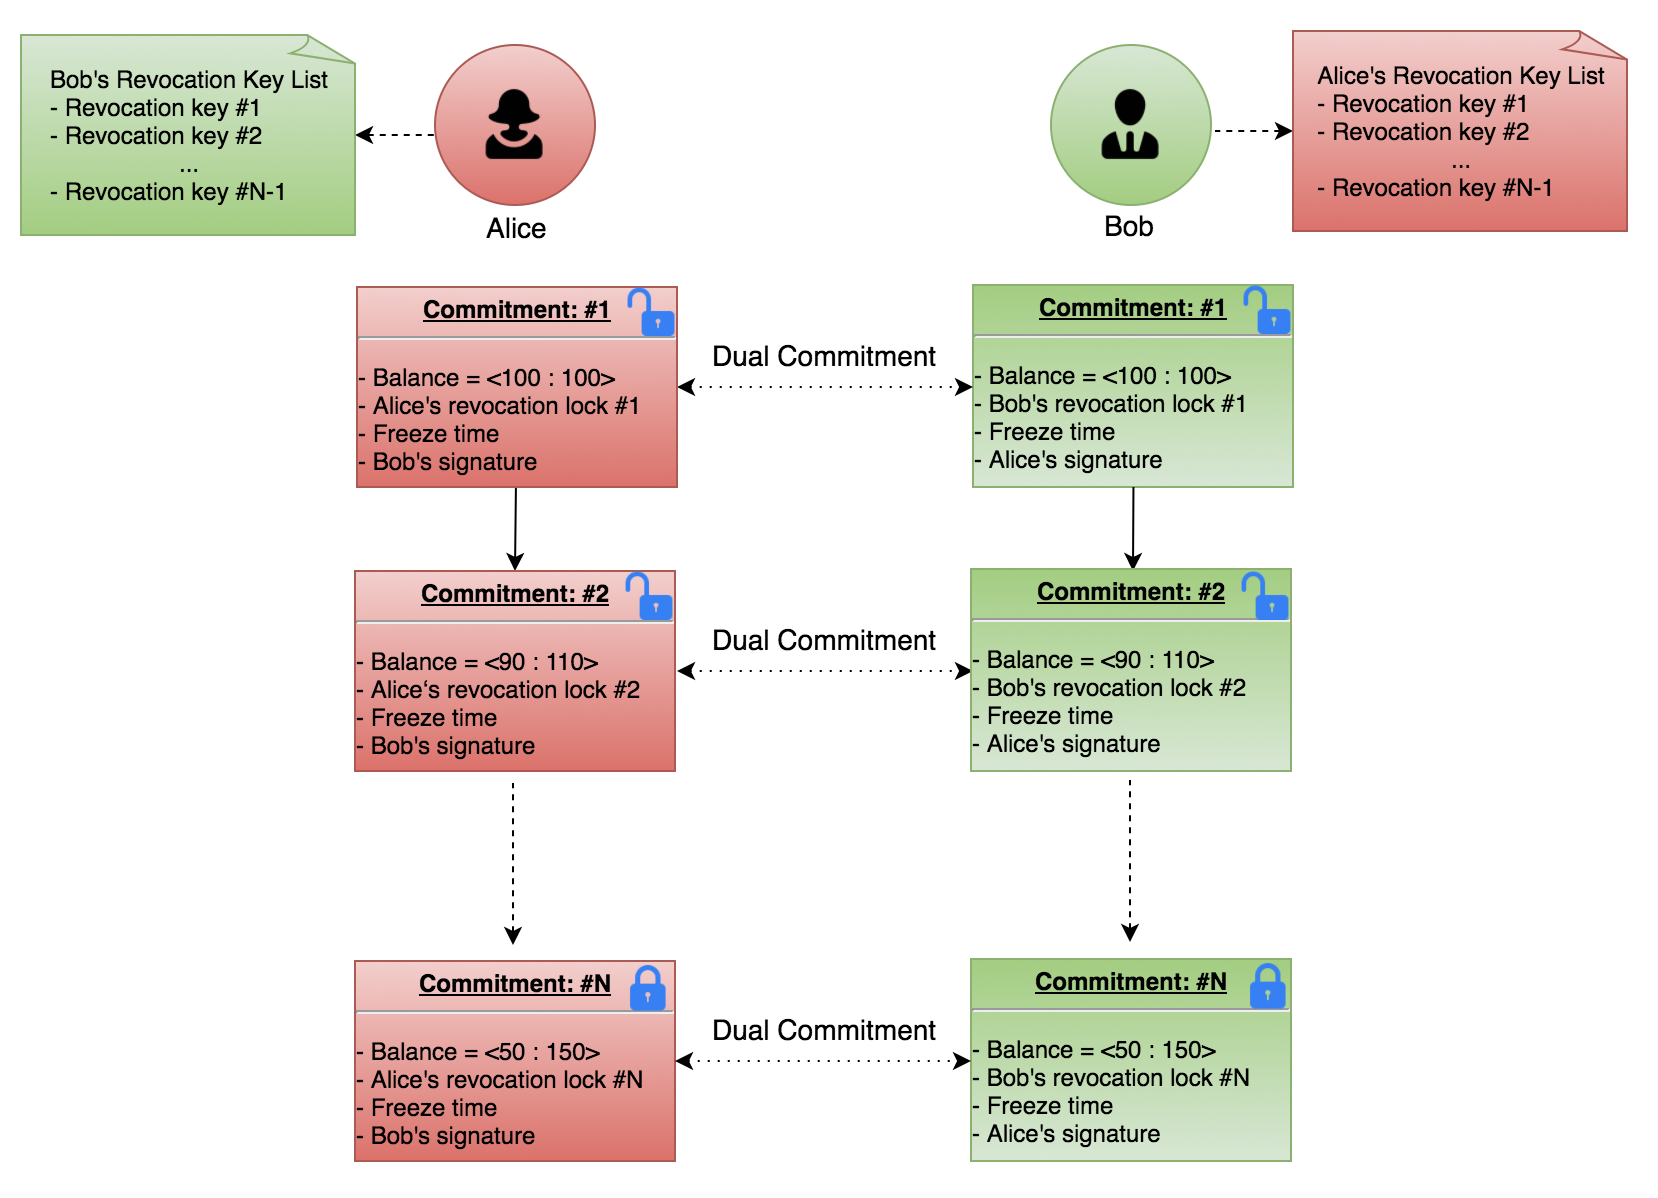
\includegraphics[width=12cm, keepaspectratio]{../images/dual_rsmc_3.png}
    \caption{RSMC 承诺方案}
    \label{fig:A_rsmc_4}
\end{figure}

\subsubsection{承诺方案兑现,关闭支付通道}
达成共同承诺之后,任何一方可以选择在任何时候向虚拟银行提交最新的承诺方案,请求兑现双方的资产。
还是接着上面的例子来讲。假设 Alice 要左侧提交编号为 N 的承诺方案,其中资产分配方案为: [50, 150]。
此方案里已经有了 Bob 的签名,Alice 需要再加上自己的签名就可以广播的网络上,调用虚拟银行智能合约中的 cashRsmc() 方法,请求最终结算资产。

下面是 cashRsmc() 函数的源码,它接受5个参数,分别是:
\begin{itemize}
    \item sequence: 承诺方案的编号
    \item balances:Alice 和 Bob 最终的资产分配方案,此例中为:[50, 150]
    \item revocationLock: 编号为N,进攻方为 Alice 的撤销锁
    \item freezeTime: 诚信保证金的冻结时间
    \item defenderSignature:防御方,也就是 Bob 对此承诺方案的签名。证明 Bob 认可此承诺方案的所有配置。
\end{itemize}

rsmc() 首先检查所有输入参数是否有效,包括以下内容:

\begin{itemize}
    \item 当前虚拟银行出于 Running 状态
    \item 撤销锁不是黑洞地址
    \item 资产总额保持一致
    \item 识别进攻方的身份,并且验证防御方的签名
\end{itemize}

\begin{lstlisting}[caption={兑现RSMC共同承诺}, label={lst:cashRsmc}]
/**
 * @notice Virtual bank cash a RSMC commitment which is submitted by Alice or Bob.
 * @param sequence          The sequence number of the commitment.
 * @param amounts           The amounts of new balance sheet
 * @param revocationLock    The revocation lock for attacker's findelity bond.
 * @param freezeTime        The freeze time for attacker's findelity bond.
 * @param defenderSignature The defender's signature.
 */
function cashRsmc(uint32 sequence, uint256[2] amounts, address revocationLock, 
                  uint freezeTime, bytes defenderSignature) 
        external isRunning() validAddress(revocationLock) {
    require((amounts[0] + amounts[1]) == (_clients[0].amount + _clients[1].amount), 
    "Total amount doesn't match.");
    // identify attacker's index
    uint8 attacker = findAttacker();
    uint8 defender = 1 - attacker;
    // check defender's signature over sequence, revocation lock, new balance sheet, freeze time
    bytes32 msgHash = keccak256(abi.encodePacked(address(this), sequence, 
    amounts[0], amounts[1], revocationLock, freezeTime));
    require(checkSignature(msgHash, defenderSignature, _clients[defender].addr));
    uint requestTime = now;
    emit CommitmentRSMC(sequence, NAMES[attacker], amounts[0], amounts[1], 
    revocationLock, requestTime, freezeTime);
    _doCommitment(sequence, attacker, amounts, revocationLock, requestTime, freezeTime);
}
\end{lstlisting}

验证无误之后,调用内部函数 \_doCommitment() 执行资产的分配。
然后根据\textbf{防御方优先结算}的原则,先返还 Bob 的 150 美金资产。
把 Alice 的 50 美元资产暂时冻结,从当前开始计算冻结时间,虚拟银行进入 Auditing 状态。

\begin{lstlisting}[caption={执行共同承诺}, label={lst:_doCommitment}]
/**
 * @notice Virtual bank settle defender's fund immediately, and freeze the attacker's 
 *         fund as fidelity bond.
 * @param sequence          The sequence number of the commitment.
 * @param attacker          The attacker's index.
 * @param amounts           Virtual bank settle fund according to this balance sheet
 * @param revocationLock    The revocation lock for attacker's findelity bond.
 * @param requestTime       The time when virtual bank recieves the commitment, ie. 
 *                          the start time of fidelity bond freezing.
 * @param freezeTime        How long attacker's findelity bond will be freezed.
 */
function _doCommitment(uint32 sequence, uint8 attacker, uint256[2] amounts, 
                       address revocationLock, uint requestTime, uint freezeTime) 
            internal {
    _commitment.sequence = sequence;
    _commitment.attacker = attacker;
    _commitment.revocationLock = revocationLock;
    _commitment.requestTime = requestTime;
    _commitment.freezeTime = freezeTime;
    _commitment.amounts[0] = amounts[0];
    _commitment.amounts[1] = amounts[1];
    
    state = State.Auditing;
    emit VirtualBankAuditing();
    
    // send fund to defender now
    uint8 defender = 1 - attacker;
    _clients[defender].addr.send(amounts[defender]);
    
    emit Withdraw(sequence, NAMES[defender], _clients[defender].addr, amounts[defender]);
    emit FreezeFidelityBond(sequence, NAMES[attacker], amounts[attacker], revocationLock, 
    requestTime + freezeTime);
}
\end{lstlisting}

\subsubsection{诚信保证金}
前面的一章提到,设立诚信保证金的目的是防止进攻方作弊,提交已经被撤销的承诺方案。
比如对于 Alice 来讲,编号为 \#2 的承诺方案更有利,她可以获得 120 美元。
共同承诺的兑现相当于瓜分银行的总资产,这是一种零和博弈。
假设 Alice 和 Bob 都是理性的决策者,无论谁作为进攻方主动分割资产,都不会做出于对方有利,于己方不利的决策。
所以在承诺方案的处理过程中,冻结进攻方的资产,同时防御方通过虚拟银行智能合约释放的事件 CommitmentRSMC() 可以得知承诺方案的编号,而且有充分的时间审查此承诺方案释放过期。

正常情况下,Alice 是诚实的,资产编号为最新的,Bob 不会对承诺方案有异议。
在冻结期满之后,Alice 可以调用 withdrawByAttacker() 函数赎回被冻结的资产。
此函数的源码如下。处理逻辑比较简单,首先检查虚拟银行当前状态是 Auditing, 而且此消息是由进攻方发出的。
如果检查冻结时间已满,那么将诚信保证金发给进攻方,同时虚拟银行的状态变成 Closed。

\begin{lstlisting}[caption={锁定时间过后,进攻方取回诚信保证金}, label={lst:withdrawByAttacker}]
/**
 * @notice After freezing time, attacker withdraws his fidelity bond.
 */
function withdrawByAttacker() external isAuditing() onlyAttacker(msg.sender) {
    require(now >= _commitment.requestTime + _commitment.freezeTime);
    state = State.Closed;
    emit VirtualBankClosed();

    // send fidelity bond back to attacker
    uint attacker = _commitment.attacker;
    uint256 amount = _commitment.amounts[attacker];
    msg.sender.send(amount);
    emit Withdraw(sequence, NAMES[attacker], msg.sender, amount);
}
\end{lstlisting}

但是如果 Alice 不是诚实的,比如说她提交了编号为 \#2 的承诺方案。
由于 Bob 保存有编号 \#1 到 \#(N-1) 的所有撤销锁私钥,Bob 可以使用其中的 \#2 号私钥签名,调用 withdrawByDefender() 在冻结期未满的时候取出诚信保证金。
下面是 withdrawByDefender() 的源码。此函数先确定虚拟银行当前的状态是 Auditing,而且此消息是防御方发出的。
然后验证撤销锁的签名是否匹配,验证成功之后将诚信保证金发给防御方。

抢先赎回需要使用豁免私钥签名,此豁免私钥是由 Alice 创建的,不同的支付对应不同的豁免私钥。
在每一次支付的时候,Alice 要向 Bob 发送上一次支付对应的豁免私钥。
Bob 获得此私钥之后,可以相信 Alice 已经放弃了上次支付对应的资产分配方式。具体的操作过程请参考 RSMC 协议。

\begin{lstlisting}[caption={锁定时间内,防御方取出诚信保证金}, label={lst:withdrawByDefender}]
/**
 * @notice Defender solve the revocation lock, withdraws attacker's fidelity bond as penalty.
 * @param revocationSignature  Defender's signature to open the revocation lock.
 */
function withdrawByDefender(bytes revocationSignature) 
        external isAuditing() onlyDefender(msg.sender) {
    uint attacker = _commitment.attacker;
    uint defender = 1 - attacker;
    
    // check signature for revocation lock
    bytes32 msgHash = keccak256(abi.encodePacked(address(this), _commitment.sequence));
    require(checkSignature(msgHash, revocationSignature, _commitment.revocationLock));
    emit RevocationLockOpened( _commitment.sequence, now, _commitment.revocationLock);
    
    // Close virtual bank;
    state = State.Closed;
    emit VirtualBankClosed();
    
    // send fidelity bond to defender
    uint256 amount = _commitment.amounts[attacker];
    msg.sender.send(amount);
    emit Withdraw(sequence, NAMES[defender], msg.sender, amount);
}
\end{lstlisting}

无论是 Alice,还是 Bob 取出冻结的资产,虚拟银行都进入关闭状态,对应的支付通道随之也关闭。

\subsection{HTLC 承诺方案}
在 \ref{sec:htlc} 节已经解释过 HTLC 承诺方案的含义,是在 RSCM 的基础上又增加了 Hash 锁与时间锁。
下面使用 \ref{sec:htlc_pay} 节的例子,再结合虚拟银行智能合约来解释如何使用 HTLC 承诺方案在支付路径中传递价值。
这个过程可以分解为3个阶段:
\begin{enumerate}
    \item \textbf{准备阶段}:此阶段要确定支付路径,要链接哪些支付通道,每一段支付通道中的余额是否充足。最终支付的双方要协商 Hash 锁,并且预留足够的时间锁长度。
    \item \textbf{向前传递 HTLC 承诺方案}:此阶段从支付的发送方开始,逐步在每一个支付通道建立 HTLC 承诺方案,一直到接收方为止。这个过程也是传递 Hash 锁的过程。
    \item \textbf{后向传递 Hash 锁暗语}: 从接收方开始,逐个通道公开 Hash 锁的暗语,完成 HTLC 承诺方案的支付条件,并且更换新的 RSMC 承诺方案。
\end{enumerate}

下面按照这三个阶段的顺序,介绍实现的细节。

\subsubsection{准备阶段}

如图 \ref{fig:A_channels} 所示,假设Alice 要向 Carol 支付 10美元,他们打算通过 Bob 作为中间人传递支付。Carol 生成了随机数 R,把对应的 Hash 值 H = hash(R) 发送给 Alice。

\begin{figure}[h!]
    \centering
    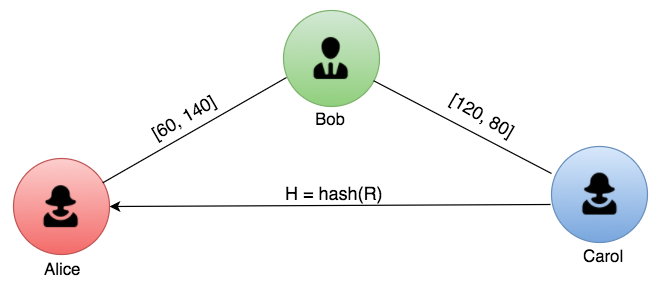
\includegraphics[width=8cm, keepaspectratio]{../images/channels.png}
    \caption{支付路径}
    \label{fig:A_channels}
\end{figure}


当前 Alice 和 Bob 之间的承诺分配方案的编号是\#N,资产分配方式是:[60, 140]。

\begin{figure}[h!]
    \centering
    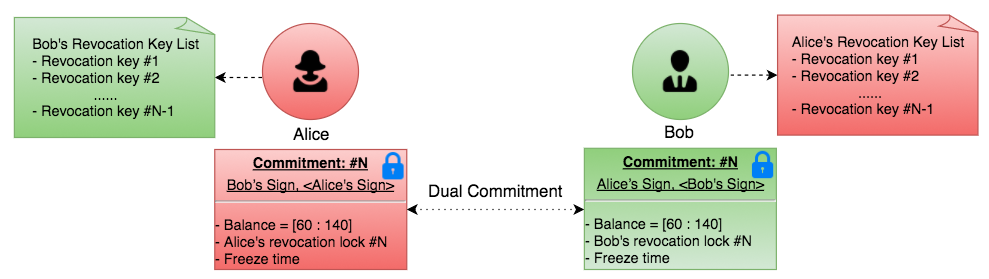
\includegraphics[width=12cm, keepaspectratio]{../images/alice_bob_1.png}
    \caption{Alice-Bob 之间支付通道状态}
    \label{fig:A_alice_bob_1}
\end{figure}

同时,Bob 和 Carol 之间的承诺分配方案编号是 \#M, 资产分配方式是:[120, 80]。

\begin{figure}[h!]
    \centering
    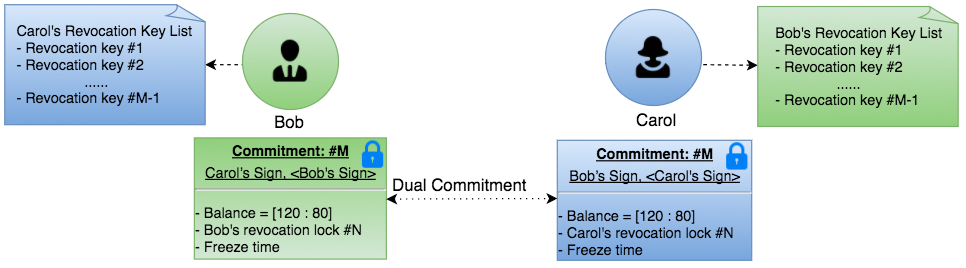
\includegraphics[width=12cm, keepaspectratio]{../images/bob_carol_1.png}
    \caption{Bob-Carol 之间支付通道状态}
    \label{fig:A_bob_carol_1}
\end{figure}

\subsubsection{前向传递 HTLC 承诺方案}
首先 Alice 和 Bob 先建立 HTLC 承诺方案,如下图 \ref{fig:A_alice_bob_2} 所示。
新的 HTLC 方案编号为 N+1。在此承诺中,双方约定,如果 Bob 能在未来\textbf{2小时}之内,公开Hash 锁对应的暗语 R,
那么就按照 [50, 150] 的方式重新分配资产,等价于 Alice 向 Bob 支付 10 美元。
否则还是按照 [60, 140] 的方式分配资产。同时双方都统一撤销编号为 N 的旧承诺。

\begin{figure}[h!]
    \centering
    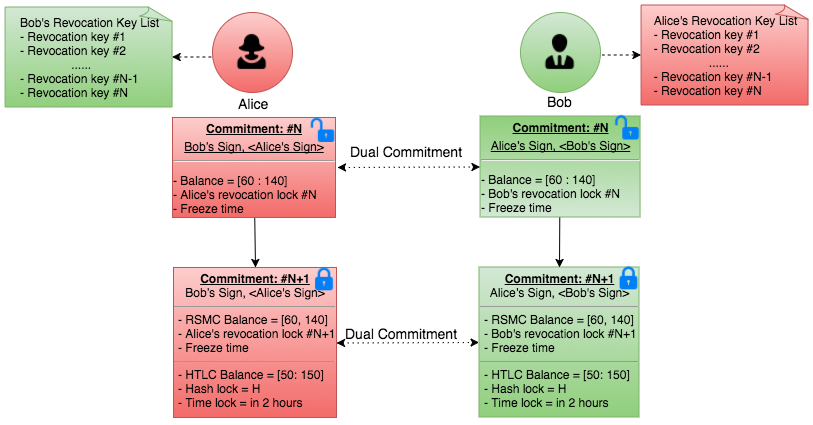
\includegraphics[width=12cm, keepaspectratio]{../images/alice_bob_2.png}
    \caption{Alice-Bob 创建新的 HTLC 承诺方案}
    \label{fig:A_alice_bob_2}
\end{figure}

Bob 和 Alice 协商后,拿到 Hash 锁以及锁定的时间,然后转过身 和 Carol 也建立 HTLC 承诺方案,如下图 \ref{fig:A_bob_carol_2} 所示。
新的 HTLC 方案编号为 M+1。在此承诺中,双方约定,如果 Carol 能在未来\textbf{1小时}之内,公开 Hash 锁对应的暗语 R,那么就按照 [110, 90] 的方式重新分配资产,等价于 Bob 向 Carol 支付了 10 美元。
否则还是按照 [120, 90] 的方式分配资产。同时双方都统一撤销编号为 M 的旧承诺。

需要注意的是,这里的时间锁为 1小时,前一个时间锁为 2小时。这是为了保证 Bob 从 Carol 那里获得 Hash 锁的暗语 R 之后,有足够长的时间在传递给 Alice。否则一旦逾期,就算拿到 R 也没有意义了。

\begin{figure}[h!]
    \centering
    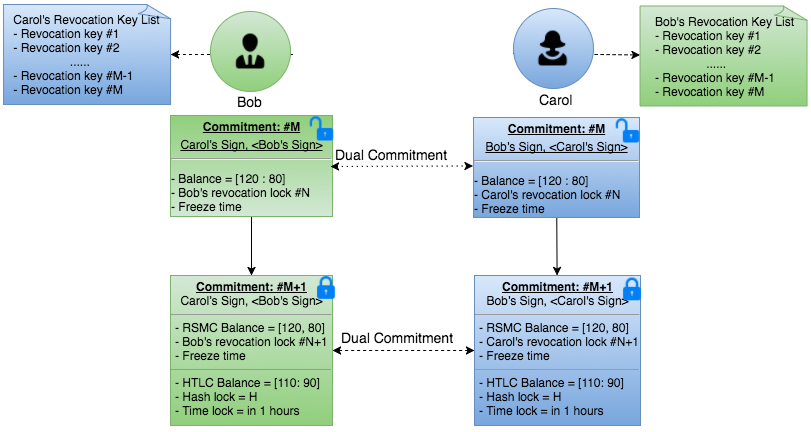
\includegraphics[width=12cm, keepaspectratio]{../images/bob_carol_2.png}
    \caption{Bob-Carol 创建新的 HTLC 承诺方案}
    \label{fig:A_bob_carol_2}
\end{figure}

\subsubsection{后向传递 Hash 锁暗语}
由于 Carol 知道暗语 R,在约定的 1小时之内把 R 的值公开给 Bob。Carol 有两种方式公开 R。
一是私下里把 R 发送给 Bob,第二种是把 HTLC 承诺方案 \#M+1 提交给虚拟银行结算,由虚拟银行公布 R 的值。

在第一种情况下,Bob 和 Carol 都认可新的资产分配方案 [120, 80],他们可以再创建一个长期有效的 RSMC 承诺方案 \#M+2,同时撤销临时性的 HTLC 承诺方案 \#M+1,如下图 \ref{fig:A_bob_carol_3} 所示。

\begin{figure}[h!]
    \centering
    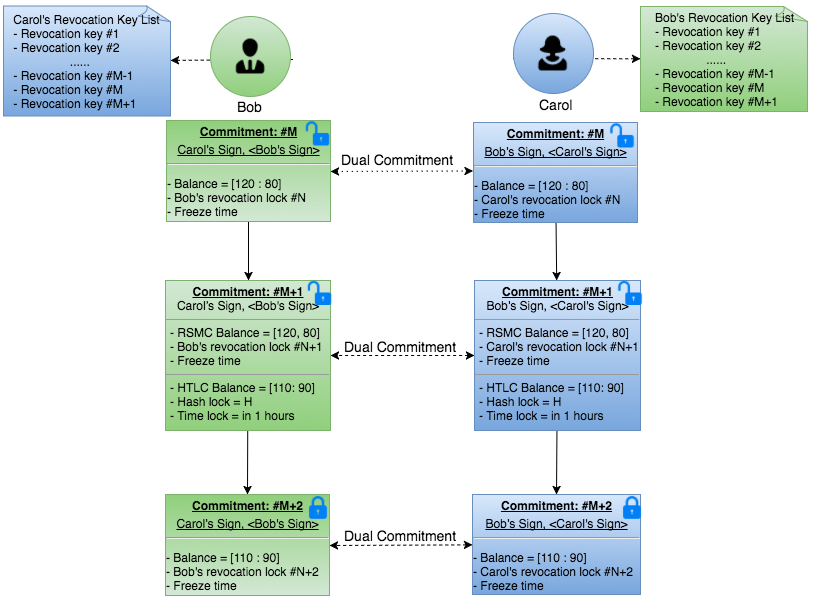
\includegraphics[width=12cm, keepaspectratio]{../images/bob_carol_3.png}
    \caption{Carol 公开暗语 R,创建无期限的 RSMC 承诺方案替代临时的 HTLC 承诺方案}
    \label{fig:A_bob_carol_3}
\end{figure}

如果是第二种情况,Carol 在HTLC承诺方案 \#M+1 中补上自己的签名,然后调用虚拟银行智能合约的 cashHtlc() 方法,请求虚拟银行结算。
对应的源代码如下。cashHtlc() 函数会检查时间锁是否预期,如果预期那么按照原来的 [120, 80] 结算资产。
如果没有预期,而且Hash锁也匹配,那么按照新的 [110, 90] 结算资产。

\begin{lstlisting}[caption={兑现HTLC共同承诺}, label={lst:cashHtlc}]
/**
 * @notice Virtual bank cash a HTLC commitment which is submitted by Alice or Bob.
 * @param sequence          The sequence number of the commitment.
 * @param rsmcAmounts       Virtual bank settle fund according to this balance sheet if 
 *                          HTLC time lock expire.
 * @param revocationLock    The revocation lock for attacker's findelity bond.
 * @param freezeTime        The freeze time for attacker's findelity bond.
 * @param hashLock          The hash lock in HTLC commitment.
 * @param preimage          The pre-image for the hash lock.
 * @param timeLock          The time lock in HTLC commitment.
 * @param htlcAmounts       Virtual bank settle fund according to this balance sheet if 
 *                          both time lock and hash lock are satisfied.
 * @param defenderSignature The defender's signature.
 */
function cashHtlc(uint32  sequence,        uint256[2] rsmcAmounts, 
                  address revocationLock,  uint       freezeTime, 
                  bytes32 hashLock;        bytes      preimage;
                  uint    timeLock;        uint[2]    htlcAmounts;
                  bytes   defenderSignature) 
         external isRunning() validAddress(revocationLock){

    // check rsmcAmounts
    require((rsmcAmounts[0] + rsmcAmounts[1]) == (_clients[0].balance + _clients[1].balance), 
            "rsmcAmounts total amount doesn't match.");
    
    // check htlcAmounts
    require((htlcAmounts[0] + htlcAmounts[1]) == (_clients[0].balance + _clients[1].balance), 
            "htlcAmounts total amount doesn't match.");
    
    // identify attacker's index
    uint8 attacker = findAttacker();
    uint8 defender = 1- attacker;
    
    // check defender signature over parameters
    bytes32 msgHash = keccak256(abi.encodePacked(address(this), sequence, rsmcAmounts[0], 
                        rsmcAmounts[1], revocationLock, freezeTime, hashLock, 
                        timeLock, htlcAmounts[0], htlcAmounts[1]));
    require(checkSignature(msgHash, defenderSignature, _clients[defender].addr));
    
    uint requestTime = now;
    emit CommitmentHTLC(sequence, NAMES[attacker], 
                rsmcAmounts[0], rsmcAmounts[1], revocationLock, requestTime, freezeTime,
                hashLock, preimage, timeLock, htlcAmounts[0], htlcAmounts[1]);
    
    // check time lock
    if (requestTime >= timeLock){
        emit TimeLockExpire(sequence, requestTime, timeLock);
        // if time lock expire, handle this commitment as RSMC
        _doCommitment(sequence, attacker, rsmcAmounts, revocationLock, requestTime, freezeTime);
    } else if {
        // check msgHash lock
        require (keccak256(preimage) == hashLock);
        emit HashLockOpened(address(this), sequence, hashLock, preimage, requestTime);
        // if both time lock and hash lock are satisfied, handle this commitment as HTLC
        _doCommitment(sequence, attacker, htlcAmounts, revocationLock, requestTime, freezeTime);
    }
}
\end{lstlisting}

无论是哪一种方式,Bob 都向 Carol 支付了 10 美元,同时获得了暗语 R。
而且与Alice 之间的承诺方案至少还有1个小时的时间,有足够的时间公示 R,从 Alice 那里获得 10 美元的补偿。
同样,Bob 也有两种方式公开 R。如果选择私下里发送给 Alice,就需要再生成新的RSMC 承诺方案\#N+2, 并且撤销 HTLC 承诺方案\#N+1,最终的结果如下图 \ref{fig:A_alice_bob_3} 所示:
\begin{figure}[h!]
    \centering
    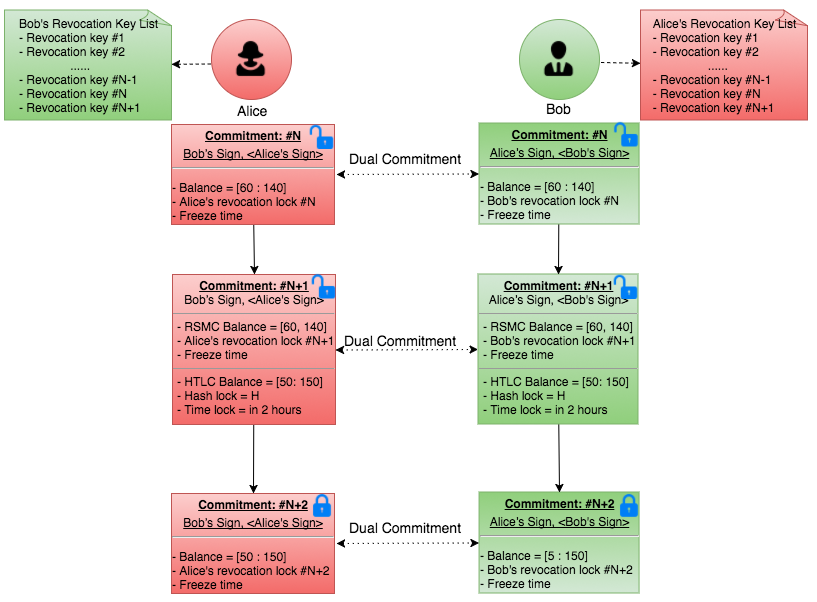
\includegraphics[width=12cm, keepaspectratio]{../images/alice_bob_3.png}
    \caption{Bob 公开暗语 R,创建无期限的 RSMC 承诺方案替代临时的 HTLC 承诺方案}
    \label{fig:A_alice_bob_3}
\end{figure}

至此,Alice 通过 Bob提供的过度资金向 Carol 支付了 10 美元。整个支付过程完毕。
\end{appendices}
